
%%%%%%%%%%%%%%%%%%%%%%% file typeinst.tex %%%%%%%%%%%%%%%%%%%%%%%%%
%
% This is the LaTeX source for the instructions to authors using
% the LaTeX document class 'llncs.cls' for contributions to
% the Lecture Notes in Computer Sciences series.
% http://www.springer.com/lncs       Springer Heidelberg 2006/05/04
%
% It may be used as a template for your own input - copy it
% to a new file with a new name and use it as the basis
% for your article.
%
% NB: the document class 'llncs' has its own and detailed documentation, see
% ftp://ftp.springer.de/data/pubftp/pub/tex/latex/llncs/latex2e/llncsdoc.pdf
%
%%%%%%%%%%%%%%%%%%%%%%%%%%%%%%%%%%%%%%%%%%%%%%%%%%%%%%%%%%%%%%%%%%%


\documentclass[runningheads,a4paper]{llncs}

%\usepackage{amssymb}
%\setcounter{tocdepth}{3}
%\usepackage{graphicx}
\usepackage{graphicx}
\usepackage{marvosym}

\usepackage{url}
\begin{document}

\mainmatter  % start of an individual contribution

% first the title is needed
\title{Toward Linking Grants and Grants Outcomes: Exploring the Socio-Technical Capabilities for Open Access Grant Information}

\titlerunning{Toward Linking Grants and Grants Outcomes}

\newcommand\Mark[1]{\textsuperscript#1}
\author{Marta Poblet\Mark{1}
\and Amir Aryani \Mark{2}
\and Kate Caldecott\Mark{3} \and Timos Sellis\Mark{1} }


\institute{
\Mark{1} RMIT University, \{marta.pobletbalcell,timos.sellis\}@rmit.edu.au\\
\Mark{2} Australian National University, amir.aryani@anu.edu.au\\
\Mark{3} Our Community - Australian Institute of Grants Management, kcaldecott@ourcommunity.com.au\\
}

\authorrunning{Toward Linking Grants and Grants Outcomes}


\toctitle{Lecture Notes in Computer Science}
\tocauthor{Authors' Instructions}
\maketitle

\begin{abstract}
Grants are the steam engine of the research enterprise. Each year, billions of taxpayer�s money and philanthropy contributions enable new research projects across the world. However, despite the significant investment of public money in the research and innovation, the information about these publicly funded projects and their impact is hidden behind disconnected, undiscoverable and inaccessible information systems. In this paper, we discuss the need for a coordinated effort toward enabling open access to grant information; in addition, as a case study, the authors describe the recent developments toward open access policy in Australia and supporting social-technical capabilities. Furthermore, this paper proposes a framework for coordinating technical and policy-making efforts toward linking grants to grant outcomes (publications, patents, research data, etc.). 
\end{abstract}


\section{Introduction}
Competitive grant programs release billions of dollars in annual rounds worldwide. Yet, as Lane has recently put it, ``answers to the question about the returns on investment have been patchy'' \cite{Lane2014}. This observation is applicable to many contexts. In Europe, where the current H2020 Framework Program will release nearly \EUR{80} billion for research and innovation over the next seven years, policy reports acknowledged that evaluation ``has been closely tied to the programming cycle'' and the available records ``tells us too little about wider or longer-term impacts or about the achievement of political and policy objective'' \cite{Arnold}. To face similar challenges, a number of countries are currently developing an open data infrastructure to evaluate the impact of government-funded scientific research. In the US, the STAR METRICS project is conceived as ``a partnership between science agencies and research institutions to document the outcomes of science investments to the public''\footnote{See \url{https://www.starmetrics.nih.gov} }. In Australia, the two federal funding bodies (ARC and NHMRC) have recently issued open access mandates as a step towards an ecosystem of open research. 

Yet, when it comes to private grantmaking, research and evaluation of the impact of funding allocated to scientific research is even more limited. The existing literature is domain specific and does not allow for cross-country analysis \cite{Ardoin2012,Reckhow2012,Bernstein2013,Caisley2013}. One of the biggest impediments is the absence of an adequate data infrastructure. Recent research on the impact of US foundations� grants on the education system has noted that ``some foundations report all of their grants on their websites or in their annual reports, but many do not. This information does not become publicly available until foundation tax returns are released, often two years after the grants were distributed'' \cite{Reckhow2012}. 

A number of recent initiatives have been recently launched to address these challenges. In the US, fifteen of the largest foundations have partnered together to open up their grantmaking data in a transparency-centered website, Glasspockets.org\footnote{See \url{http://www.glasspockets.org}}. According to Judith Rodin, president of the Rockefeller Foundation, the platform ``liberates grants data from the confines of a single foundation and brings knowledge sharing to the fore'' (Foundation Center 2012). Data is published in an open format, coded in open geographic standards, and licensed under Creative Commons licenses.

This paper discusses the need for a coordinated effort towards enabling open access to grant information. For the purposes of the paper we broadly define grants as the money awards given by public or private institutions to either individuals or organisations (grant recipients or grantees) to carry out a specific activity and deliver identifiable outputs. The grantmaking process is a structured cycle of events usually including an open call, an application phase, a decision-making process determining successful candidates (grantees), an execution phase, and an evaluation phase. All these grantmaking cycle events are able to generate grant data (i.e. on funding organisations, grant participants, funding amounts, domains being funded, geographic scope, etc.). Grant data is different from �research data�. In a data management guideline\footnote{See \url{http://ands.org.au/guides/what-is-research-data.html}} by Australian National Data Service, research data is defined as the form of facts, observations, images, computer program results, recordings, measurements or experiences on which an argument, theory, test or hypothesis, or another research output is based. Research data may be numerical, descriptive, visual or tactile. It may be raw, cleaned or processed, and may be held in any format or media.

The rest of this paper is organised as follows: Section 2 proposes a framework for coordinating technical and policy-making efforts toward linking grants to grant outcomes. Recent developments towards an open access policy in Australia are covered in Section 3, and finally Section 4 presents concluding remarks.

\section{Framework: Linking Grants to Research Outcome}
The proposed framework describes the type of connections between research grant information and other data elements in the research ecosystem. This framework is mainly aimed to highlight the gaps at the national and international research infrastructures and discuss the required social and technical capabilities in this domain.


Providing open access information about the research grants is one of the key enablers for creating a connected research ecosystem and treatability of research outcomes. There are three main motivations for creating such a connected ecosystem:

\begin{itemize}  \itemsep0.5em
\item \emph{Better discovery of research outcomes:} improving discovery of research outcomes can lead to new collaboration opportunities, and potentially new research and innovations.
\item \emph{Better return on investment:} the vision of scientific community that does not waste resources on recreating research data has been the objective of many policy makers and funding agencies. Vice-President of the EU Commission and Responsible for the Digital Agenda Neelie Kroes envisages such community in the introduction of the Final Report of the High Level Expert Group on Scientific Data (HLSGSC 2010). Providing open access to research grant information and their outcomes (including publication and data) enables better reuse of research outcomes, hence better return of investment.
\item \emph{Better transparency and open access compliance:} given most research grants are funded through public money (federal funding, or philanthropic contributions) in most cases compliance with open data policies is a requirement for awarded grants. However, the level of compliance at this stage does not extend to machine readable interfaces, leading to unnecessary effort by staff at research institutions to manually track and re-enter this information in institutional repositories, research management systems and institution profiles. In addition, it significantly hinders the effort of systematic analysis of grant data and interoperability between research information systems.
\end{itemize}

\begin{figure}[h]
\begin{center}
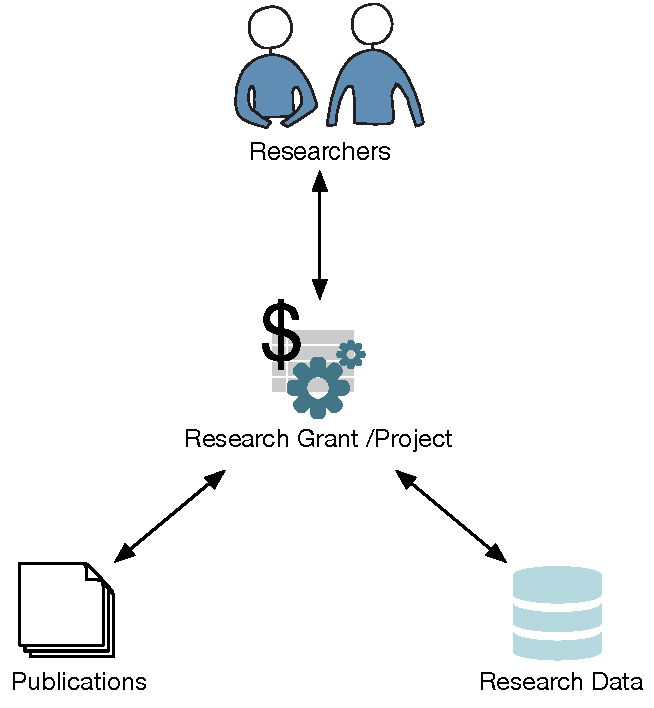
\includegraphics[width=0.5\columnwidth]{grantlinks.pdf}
\end{center}
\label{fig:Figure1}
\caption{The connections between grants, grantee, publications and research data is essential to make the grant data and research outcome discoverable and reusable.}
\end{figure}

\noindent
In order to achieve connected, discoverable, reusable and (openly) accessible grant data, this paper stresses the need for the following connectivity (Figure~1):

\begin{itemize} \itemsep0.5em
\item \emph{Linking grants to grant investigators (grantees):} the connections between grant investigators and their awarded grants is vital to make the research outcomes discoverable and reusable.  Discoverability of these connections enables further research collaborations and innovation. The main technical barrier in this area is author name disambiguation. It is common for researchers to collaborate across universities, countries and continents. In this vast environment, it is also common to find people with similar names. Hence, without adopting international author identifiers (such as the ones provided by ISNI, ORCID, ResearchID) linking grants to researchers can be a technical challenge.
\item \emph{Linking grants to publications:} one of the most direct approaches to measure and understand the outcome of research projects is through the peer-reviewed publications. The publication outcome from grants is often considered as one of the major indications of research impact. The connectivity between publications and grants improves the discoverability of the research, and leads to better citation and recognition of the work. There has been national and international efforts in this area such as recent effort by CrossRef  for establishing FundRef service, and OpenAire  in Europe; however, there social and technical limitation that affect these services including (not limited to): lack of unique and persistent identifiers for research grants, lack of consistent acknowledgment of grants in publications and limited open access culture and capabilities.
\item \emph{Linking grants to research data: }the relation between grants and research data is an important component in improving discoverability and reusability of research data. The connection between grants and datasets enables researchers to find the data derived from high impact research projects and promotes reuse and credibility of research data; in addition, the funding agencies have a new focus on open access for publications, and similar trend can be expected for research data. The main social and technical challenges in linking grants to research data is the shortfall in the culture of data citation, inconsistent open access policies for research data, lack of unique persistent identifiers for research grants, and limited open access capabilities by research data repositories. 
\end{itemize}

\noindent
Moreover, this technical framework will not operate in a social and legal vacuum. Rather, an ecosystem of open access grant information will need to address a number of legal and ethical issues related to data protection, privacy, or copyright (i.e. which data protection and privacy regulations/policies apply or need to be designed? Which licensing options are available? Which countries or jurisdictions allow voluntary relinquishment of copyright?). Likewise, decisions on which are the most adequate open access publishing models are almost inevitably controversial. A recent example of this is the policy introduced by Research Councils UK (RCUK) in April 2013\footnote{See \url{http://www.rcuk.ac.uk/research/openaccess} } supporting the so-called ``gold'' open access model over the ``green'' model \cite{Kingsley2013}.   

\section{Open Access in Australia}
Australia is one of the world-leading countries in promoting open-access policies. In recent years a number of institutions have implemented open-access mandates in different areas, notably in government and research. The National Health and Medical Research Council (NHMRC) and the Australian Research Council (ARC) released their Open Access mandates in 2012 and 2013 respectively. Both policies require that any publications arising from a funded research project must be deposited into an open access institutional repository within a 12 month period from the date of publication. Researchers are also encouraged to make accompanying datasets available open access \cite{Kingsley2013}. The federally funded Australian National Data Service (ANDS) is currently delivering infrastructure and services such as Research Data Australia\footnote{Research Data Australia is a discovery service and search engine for research data from Australian institutions. See \url{researchdata.ands.org.au}} and the Australian Research Data Commons. More recently, ANDS has developed the Research Grants API\footnote{See \url{http://researchdata.ands.org.au/developers}}, that enables discovery of published research grants based on their title, or relationship to specific individuals or institutions. 

As a result of federal investment, all Australian universities have nowadays a repository, and one third (13 of 39) of them have an open access policy\footnote{See \url{http://aoasg.org.au/open-access-policies}}. Yet, as Kingsley has noted, integration remains an issue, since ``there is currently no way of extracting open access research across the country in a single database''.

Another open data initiative in Australia is the ``Collaborative Grantmaking in Western Sydne'' pilot project being run by the Australian Institute of Grantmaking (AIGM), a division  of Our Community, an Australian social enterprise. This pilot project involves 7 local Government Councils and Clubs NSW collaborating to evaluate funding effectiveness in Western Sydney (involving a combined estimate of \$9 million in grants per annum). Data collection is via the AIGM�s SmartyGrants system,  Australia�s most widely used grants management system (GMS) incorporating over 3,600 grants program from private and public grantmakers.  From there, through the AIGM�s relationships with private and public Australian Grantmakers, the goal is to extend the project creating an ethical open common data framework and establishing a public interface allowing for increased transparency and analysis by grantmakers and grantees.

Despite all the efforts at the national level to enable open access to research data in Australia, there are still limitations in socio-technical capabilities that hinder linking grants to research outcomes. Among the most salient are:

\begin{itemize}\itemsep0.5em
\item Shortfall in open access platforms for grant data: although ANDS provides an open access platform for grant data, at the time of writing this article the grant data coverage is limited only to the two major federal funding agencies (ARC and NHMRC). 
\item Shortfall in open access platforms for grant data: although ANDS provides an open access platform for grant data, at the time of writing this article the grant data coverage is limited only to the two major federal funding agencies (ARC and NHMRC). 
\item Limited coordinated approach at the national and international level to grant metadata 
\item Limited support for unique persistent identifier for research grants: ANDS supports persistent URL (PURLs) for grants and research projects; however, to date the scope of this service has not expanded beyond ARC and NHMRC grants.
\item Shortfall in the national adoption of author identifiers: the adoption of author identifiers in Australia has oscillated between ISNI (International Standard Name Identifier), ORCID and Author Identifiers provided by National Library of Australia. However, the adoption of these identifiers has not reached the required level to support a national interoperability between research management systems and enable identifying authors and grantees at across institutions yet.
\item Limited capabilities for linking grants to publications
\item Limited technical capabilities for linking research data to grants
\end{itemize}

\noindent
In addition to the open access limitations for grant data and required linking capabilities at the national level, one can argue that research is a collaborative enterprise, and for research outcomes to be reusable, a coordination effort is needed across international research institutions.

It is common that researchers collaborate or move across institutions, also grants can be awarded to more than one research institution as such linking grant data to publication and datasets requires interoperability across software platforms and administrative collaboration across research institutions. Finally, research projects can impact ongoing works or inspire new ideas through a network of research collaborators working in different continents. Hence, policy-makers, research managers, funding agencies and university administrations requires to collaborate at the international level toward an open access agenda for grant data and linking grants to research outcomes.

\section{Concluding Remarks}

This paper approaches grantmaking as a socio-technical process where coordination among national and international institutions is crucial to achieve greater levels of efficiency and impact. To date, these efforts are limited to the country level and, in most cases, to grants given by large national research organisations. Our proposed framework aims at leveraging the socio-technical value of grant data collected by large national research agencies, funding organisations and grant managers to develop an ecosystem for open access to grant information. We have briefly reviewed some promising initiatives in this line. Yet, a number of technical and legal issues need to be addressed to fully harness the potential of linked grant data for the benefit of the large scientific community. 


\begin{thebibliography}{4}

\bibitem{Ardoin2012} Ardoin, N. M., \& Bowers, A. W. (2012). Trends in Philanthropic Support: Foundation Giving in Environmental Education. The Journal of Environmental Education, 43(4), 259-273.


\bibitem{Arnold}Arnold, E. (Coord.) Understanding the Long Term Impact of the Framework Programme. Final Report To the European Commission DG Research. Available at \url{http://ec.europa.eu/research/evaluations/pdf/archive/other_reports_studies_and_documents/long_term_impact_of_the_fp.pdf}

\bibitem{Reckhow2012}Reckhow, S. (2012). Follow the money: How foundation dollars change public school politics. Oxford University Press.

\bibitem{Bernstein2013}Bernstein, M., Desy, N. M., Matache, B. A., McKinley, T. O., \& Harvey, E. J. (2013). A Ten-Year Analysis of the Research Funding Program of the Orthopaedic Trauma Association. The Journal of Bone \& Joint Surgery, 95(19), e142-1.

\bibitem{Caisley2013}Caisley, V., Codd, G., Isa, L., Seymour, S., Southee, R., Van den Broek, V., \& Wilson, K. (2013). The impact of grant funding on communities in New Zealand: a case study. Available at \url{http://www.lionfoundation.org.nz/Files/lionfoundation/berl/MasseyCaseStudy.pdf}

\bibitem{Lane2014}Lane, J. 2014 (July 22). How to better allocate research money and fix a flawed system. The conversation, \url{http://theconversation.com/how-to-better-allocate-research-money-and-fix-a-flawed-system-28593}

\bibitem{HLSGSD2010}HLSGSD (2010) Riding the wave: How Europe can gain from the rising tide of scienti�c data. Final Report of the High Level Expert Group on Scientific Data. Available at \url{http://cordis.europa.eu/fp7/ict/e-infrastructure/docs/hlg-sdi-report.pdf}
  
\bibitem{Kingsley2013}Kingsley, D. (2013, Sep. 17). UK�s open access policies have global consequences. The Conversation. Available at \url{http://theconversation.com/uks-open-access-policies-have-global-consequences-18258} 



\end{thebibliography}


\end{document}
